%% BioMed_Central_Tex_Template_v1.06
%%                                      %
%  bmc_article.tex            ver: 1.06 %
%                                       %

%%IMPORTANT: do not delete the first line of this template
%%It must be present to enable the BMC Submission system to
%%recognise this template!!

%%%%%%%%%%%%%%%%%%%%%%%%%%%%%%%%%%%%%%%%%
%%                                     %%
%%  LaTeX template for BioMed Central  %%
%%     journal article submissions     %%
%%                                     %%
%%          <8 June 2012>              %%
%%                                     %%
%%                                     %%
%%%%%%%%%%%%%%%%%%%%%%%%%%%%%%%%%%%%%%%%%


%%%%%%%%%%%%%%%%%%%%%%%%%%%%%%%%%%%%%%%%%%%%%%%%%%%%%%%%%%%%%%%%%%%%%
%%                                                                 %%
%% For instructions on how to fill out this Tex template           %%
%% document please refer to Readme.html and the instructions for   %%
%% authors page on the biomed central website                      %%
%% http://www.biomedcentral.com/info/authors/                      %%
%%                                                                 %%
%% Please do not use \input{...} to include other tex files.       %%
%% Submit your LaTeX manuscript as one .tex document.              %%
%%                                                                 %%
%% All additional figures and files should be attached             %%
%% separately and not embedded in the \TeX\ document itself.       %%
%%                                                                 %%
%% BioMed Central currently use the MikTex distribution of         %%
%% TeX for Windows) of TeX and LaTeX.  This is available from      %%
%% http://www.miktex.org                                           %%
%%                                                                 %%
%%%%%%%%%%%%%%%%%%%%%%%%%%%%%%%%%%%%%%%%%%%%%%%%%%%%%%%%%%%%%%%%%%%%%

%%% additional documentclass options:
%  [doublespacing]
%  [linenumbers]   - put the line numbers on margins

%%% loading packages, author definitions

%\documentclass[twocolumn]{bmcart}% uncomment this for twocolumn layout and comment line below
\documentclass[doublespacing,linenumbers]{bmcart}

%%% Load packages
%\usepackage{amsthm,amsmath}
%\RequirePackage{natbib}
%\RequirePackage[authoryear]{natbib}% uncomment this for author-year bibliography
%\RequirePackage{hyperref}
\usepackage[utf8]{inputenc} %unicode support
%\usepackage[applemac]{inputenc} %applemac support if unicode package fails
%\usepackage[latin1]{inputenc} %UNIX support if unicode package fails

\usepackage{graphicx}
\usepackage{multirow}
\usepackage{dirtytalk}
\usepackage{tabularray}
\usepackage{hyperref}

%%%%%%%%%%%%%%%%%%%%%%%%%%%%%%%%%%%%%%%%%%%%%%%%%
%%                                             %%
%%  If you wish to display your graphics for   %%
%%  your own use using includegraphic or       %%
%%  includegraphics, then comment out the      %%
%%  following two lines of code.               %%
%%  NB: These line *must* be included when     %%
%%  submitting to BMC.                         %%
%%  All figure files must be submitted as      %%
%%  separate graphics through the BMC          %%
%%  submission process, not included in the    %%
%%  submitted article.                         %%
%%                                             %%
%%%%%%%%%%%%%%%%%%%%%%%%%%%%%%%%%%%%%%%%%%%%%%%%%


%\def\includegraphic{}
%\def\includegraphics{}



%%% Put your definitions there:
\startlocaldefs
\endlocaldefs


%%% Begin ...
\begin{document}

%%% Start of article front matter
\begin{frontmatter}

\begin{fmbox}
\dochead{Research}

%%%%%%%%%%%%%%%%%%%%%%%%%%%%%%%%%%%%%%%%%%%%%%
%%                                          %%
%% Enter the title of your article here     %%
%%                                          %%
%%%%%%%%%%%%%%%%%%%%%%%%%%%%%%%%%%%%%%%%%%%%%%

\title{Turning the tide: Understanding estuarine detection range variability via structural equation models}

%%%%%%%%%%%%%%%%%%%%%%%%%%%%%%%%%%%%%%%%%%%%%%
%%                                          %%
%% Enter the authors here                   %%
%%                                          %%
%% Specify information, if available,       %%
%% in the form:                             %%
%%   <key>={<id1>,<id2>}                    %%
%%   <key>=                                 %%
%% Comment or delete the keys which are     %%
%% not used. Repeat \author command as much %%
%% as required.                             %%
%%                                          %%
%%%%%%%%%%%%%%%%%%%%%%%%%%%%%%%%%%%%%%%%%%%%%%

\author[
   addressref={aff1},                   % id's of addresses, e.g. {aff1,aff2}
   corref={aff1},                       % id of corresponding address, if any
   noteref={n1},                        % id's of article notes, if any
   email={stijn.bruneel@ugent.be}   % email address
]{\inits{S}\fnm{Stijn} \snm{Bruneel}}
\author[
   addressref={aff2},
   email={jolien.goossens@ugent.be}
]{\inits{J}\fnm{Jolien} \snm{Goossens}}
\author[
   addressref={aff3},
   email={jan.reubens@ugent.be}
]{\inits{J}\fnm{Jan} \snm{Reubens}}
\author[
   addressref={aff4},
   email={ine.pauwels@inbo.be}
]{\inits{I}\fnm{Ine} \snm{Pauwels}}
\author[
   addressref={aff2},
   email={tom.moens@ugent.be}
]{\inits{T}\fnm{Tom} \snm{Moens}}
\author[
   addressref={aff1},
   email={peter.goethals@ugent.be}
]{\inits{P}\fnm{Peter} \snm{Goethals}}
\author[
   addressref={aff2,aff4},
   email={pieterjan.verhelst@inbo.be}
]{\inits{P}\fnm{Pieterjan} \snm{Verhelst}}

%%%%%%%%%%%%%%%%%%%%%%%%%%%%%%%%%%%%%%%%%%%%%%
%%                                          %%
%% Enter the authors' addresses here        %%
%%                                          %%
%% Repeat \address commands as much as      %%
%% required.                                %%
%%                                          %%
%%%%%%%%%%%%%%%%%%%%%%%%%%%%%%%%%%%%%%%%%%%%%%

\address[id=aff1]{%                           % unique id
  \orgname{Department of Animal Sciences and Aquatic Ecology, Ghent University}, % university, etc
  \street{Coupure Links 653},                     %
  \postcode{9000}                                % post or zip code
  \city{Ghent},                              % city
  \cny{Belgium}                                    % country
}
\address[id=aff2]{%
  \orgname{Biology Department, Marine Biology Research Group, Ghent University},
  \street{Krijgslaan 281},
  \postcode{9000}
  \city{Ghent},
  \cny{Belgium}
}
\address[id=aff3]{%
  \orgname{Flanders Marine Institute (VLIZ)},
  \street{Wandelaarkaai 7},
  \postcode{8400}
  \city{Ostend},
  \cny{Belgium}
}
\address[id=aff4]{%
  \orgname{Research Institute for Nature and Forest (INBO)},
  \street{Havenlaan 88, bus 73},
  \postcode{1000}
  \city{Brussels},
  \cny{Belgium}
}




%%%%%%%%%%%%%%%%%%%%%%%%%%%%%%%%%%%%%%%%%%%%%%
%%                                          %%
%% Enter short notes here                   %%
%%                                          %%
%% Short notes will be after addresses      %%
%% on first page.                           %%
%%                                          %%
%%%%%%%%%%%%%%%%%%%%%%%%%%%%%%%%%%%%%%%%%%%%%%

\begin{artnotes}
%\note{Sample of title note}     % note to the article
\note[id=n1]{Equal contributor} % note, connected to author
\end{artnotes}

\end{fmbox}% comment this for two column layout

%%%%%%%%%%%%%%%%%%%%%%%%%%%%%%%%%%%%%%%%%%%%%%
%%                                          %%
%% The Abstract begins here                 %%
%%                                          %%
%% Please refer to the Instructions for     %%
%% authors on http://www.biomedcentral.com  %%
%% and include the section headings         %%
%% accordingly for your article type.       %%
%%                                          %%
%%%%%%%%%%%%%%%%%%%%%%%%%%%%%%%%%%%%%%%%%%%%%%

\begin{abstractbox}

\begin{abstract}
Insight into the detection range of acoustic telemetry systems is crucial for both sampling design and data interpretation. The detection range is highly dependent on the environmental conditions and can consequently be substantially different among aquatic systems. Also within systems, temporal variability can be significant. The number of studies to assess the detection range in different systems has been growing, though there remains a knowledge gap in estuarine habitats. In this study, a two-month experimental set-up was used to assess the detection range variability and affecting environmental factors of an estuary. Given the expected complex interplay of different factors and the difficulties it entails for interpretation, a structural equation modelling (pSEM) approach is proposed. The detection range of this estuarine study was relatively low and variable (average 50\% detectability of 106 meters and ranging between 72 and 229 meters) compared to studies of riverine and marine systems. The structural equation models revealed a clear, yet complex, tidal pattern in detection range variability which was mainly affected by water speed (via ambient noise and tilt of the receivers), water depth and wind speed. The negative effect of ambient noise and positive effect of water depth became more pronounced at larger distances. Ambient noise was not only affected by water speed, but also by water depth, precipitation, tilt angle and wind speed. Although the tilt was affected by water speed, water depth and wind speed, most of the variability in tilt could be traced back to the receiver locations. Similarly, the receiver locations seemed to explain a considerable portion of the detection range variability. Retrospective power analyses indicated that for most factors only a minor gain in explanatory power was achieved after more than two days of data collecting. Redirecting some of the sampling effort towards more spatially extensive measurements seems to be a relevant manner to improve the insights in the performance of telemetry systems in estuarine environments. Since the low and variable detection range in estuaries can seriously hamper ecological inferences, range tests with sound sampling designs and appropriate modelling techniques are paramount. 
\end{abstract}

%%%%%%%%%%%%%%%%%%%%%%%%%%%%%%%%%%%%%%%%%%%%%%
%%                                          %%
%% The keywords begin here                  %%
%%                                          %%
%% Put each keyword in separate \kwd{}.     %%
%%                                          %%
%%%%%%%%%%%%%%%%%%%%%%%%%%%%%%%%%%%%%%%%%%%%%%

\begin{keyword}
\kwd{Passive acoustic telemetry}
\kwd{Detection range}
\kwd{Estuary}
\kwd{Structural equation modelling (pSEM)}
\kwd{Statistical power analysis}
\end{keyword}

\end{abstractbox}
%
%\end{fmbox}% uncomment this for twcolumn layout

\end{frontmatter}

%%%%%%%%%%%%%%%%%%%%%%%%%%%%%%%%%%%%%%%%%%%%%%
%%                                          %%
%% The Main Body begins here                %%
%%                                          %%
%% Please refer to the instructions for     %%
%% authors on:                              %%
%% http://www.biomedcentral.com/info/authors%%
%% and include the section headings         %%
%% accordingly for your article type.       %%
%%                                          %%
%% See the Results and Discussion section   %%
%% for details on how to create sub-sections%%
%%                                          %%
%% use \cite{...} to cite references        %%
%%  \cite{koon} and                         %%
%%  \cite{oreg,khar,zvai,xjon,schn,pond}    %%
%%  \nocite{smith,marg,hunn,advi,koha,mouse}%%
%%                                          %%
%%%%%%%%%%%%%%%%%%%%%%%%%%%%%%%%%%%%%%%%%%%%%%

%%%%%%%%%%%%%%%%%%%%%%%%% start of article main body

%%%%%%%%%%%%%%%%
\section*{Background}

Understanding the limitations of monitoring tools is key to any study design, to a correct interpretation of collected data, and to draw scientifically sound conclusions \cite{Bruneel2022SamplingDiversity,Kessel2014}. Acoustic telemetry, the use of electronic transmitter tags and receivers to study movement behavior, is advancing rapidly and is increasingly being used for multiple aquatic species at different spatial and temporal scales \cite{Alos2022TowardTracking,Matley2022GlobalTelemetry,Murray2022AProgramme}. Its technological advancement and increasing use drive the demand for sound methodologies and an improved understanding of its limitations \cite{Gupte2022AData,Kessel2014}. In acoustic telemetry studies, a key methodological aspect to consider is the detection range (i.e. the relationship between the detection probability and the distance between tag and receiver) and its variability \cite{Kessel2014}. Payne et al. (2010), for example, found that neglecting detection range variability would have led to opposite conclusions regarding the diel patterns of cuttlefish behavior \cite{Payne2010InterpretingControls}. Simulation studies have shown how ignoring detection range variability during model development can lead to large biases in parameter estimates, variable degrees of confidence in position estimates and misinterpreted animal behavior \cite{Pedersen2013, Winton2018}. In addition, studies that rely on curtains of receivers to assess whether tagged animals enter and/or leave certain areas, might confuse variables affecting passage success with variables affecting detection range and the effectiveness of the curtain to detect passing animals \cite{Bruneel2020QuantifyingSystems,Steckenreuter2017}.   

Estuaries are of particular importance for fish populations due to their functions as nursery, feeding area and migration route between freshwater and marine habitats \cite{Franco2008LifeApproach}. Different fish species at different life stages use estuaries in various ways, giving rise to a broad range of movement behaviors \cite{Potter2015TheApproach}. The diadromous European eel (\textit{Anguilla anguilla}), for example, uses selective tidal stream transport to move from its fresh water feeding habitat to its marine spawning grounds \cite{Verhelst2018}. The estuarine-dependent spotted grunter (\textit{Pomadasys commersonnii}) moves between the upper and lower estuary as a response to fluctuations in temperature and salinity \cite{Childs2008DoTelemetry}, and the piscivorous red drum (\textit{Sciaenops ocellatus}) adapts its home range to food availability \cite{Kenworthy2018MovementSeascape}. The fine-scale spatiotemporal variation in environmental conditions, inherent to the dynamic nature of estuaries, will not only affect the movement behavior of fish \cite{Childs2008DoTelemetry}, but also the detection range variability at a corresponding scale. To characterize movement behavior and disentangle it from methodological biases, a sound understanding of the detection range variability in estuaries is therefore key. Nevertheless, to our knowledge, there are no dedicated methodological studies evaluating detection range in estuaries. To ensure a sound methodological basis for future studies on estuarine detection range, the estuarine detection range and affecting variables were assessed using different data processing methods and a data analysis technique not previously applied to range studies. Additionally, given the outcomes  of this study, the suitability of traditional sampling designs for detection range assessment was evaluated using power analysis.  

Studies have identified strong tidal patterns in the performance of marine networks, underlining the importance of considering detection range variability when interpreting results \cite{Cho2016TidalDetection,Mathies2014}. However, the number of potential explanatory variables in these studies has remained limited and assessments were often restricted to exploratory wavelet analyses \cite{Cho2016TidalDetection,Mathies2014}. Regression-based models with multiple variables and interactions have been developed to understand detection range variability, yet these models did not explicitly account for causality nor distinguish between indirect and direct drivers \cite{Reubens2018}. Since insight in the actual contributors to detection range variability is crucial to decide on the sampling design, and given the broad range of potentially correlated and important variables (e.g. tilt angle of the receiver, ambient noise and water speed) in an estuarine environment, an alternative approach might provide more insight. We propose piecewise structural equation models (pSEMs). pSEMs have been used in many disciplines to test causal structures and to identify whether variables have an indirect or direct relationship with the considered response \cite{Lefcheck2016PiecewiseSEM:Systematics}. Although pSEMs have not been used in any methodological telemetry study yet, they have the potential to provide a better understanding of detection range variability and were therefore used in this study. 

In addition, although researchers have come to consider range testing as essential for any telemetry study, guidelines and practical suggestions on how to perform range tests in estuaries have been lacking. Although a general understanding of the most important factors affecting detection range in a specific type of aquatic system will already provide an important baseline \cite{Gjelland2013EnvironmentalTransmission}, it is still recommended to assess and understand the network performance in any new study area. Power analyses are standard in many scientific fields to determine the magnitude and distribution of the required sampling effort. However, to our knowledge, there have not been any methodological telemetry studies that have made use of power analyses to determine how long experiments should run and how many receivers should be used to yield statistically reliable results. Here we assessed the added value of power analyses for methodological telemetry studies using the available data and developed models.  

Once the data have been collected, they need to be processed before analysis. To determine the detection probability, detection data are often aggregated over a certain time interval to account for not precisely knowing the exact moment at which a signal is transmitted. Since the transmission rate of most acoustic tags varies randomly about the nominal delay value to avoid collisions and loss of signals, it is often difficult to estimate the exact number of submitted transmissions within a certain time frame. Therefore, if the random burst interval between signals is large and the chosen temporal resolution small, the accuracy of the performance estimates will be poor and unrealistic performance values of more than 100 \% might occur. Temporal aggregation is also often applied to align the resolution of the detection data with the resolution of the explanatory variables. However, the chosen resolution of the data does not necessarily reflect the resolution that is most appropriate to describe the variability of the detection range, which might introduce poor inferences and lack of insight in fine-scale processes. More recently, time-logging built-in tags record the exact moment at which a signal is transmitted, allowing to trace each individual detection back to its original transmission and removing the necessity to aggregate the data. Since in this study receivers with time-logging built-in tags were used, both non-aggregated \cite{Cimino2018DetectionGliders,Goossens2020MooringReceivers} and aggregated data \cite{Selby2016CanHabitat,Reubens2018,OBrien2021InfluenceBight} were available for analysis. To assess the effect of data aggregation, and therefore temporal resolution, models of both datasets were developed and compared. 

This study took place in the Permanent Belgian Acoustic Receiver Network (PBARN) which consists of receivers in the Scheldt Estuary and Belgian  part  of  the  North  Sea  (BPNS). This network is being used to monitor the behavior of multiple fish species \cite{ReubensBPNS}. Our results are of direct use for the optimization of the PBARN and the interpretation of the data it generates, but will also facilitate telemetry studies elsewhere, particularly in estuarine environments. 

In summary, the aims of this study are to (i) provide an in-depth assessment of indirect and direct drivers of detection range variability in an estuarine environment through a structural equation modelling approach (i.e. pSEMs), (ii) assess the added value of statistical power analyses and provide practical suggestions regarding the required experimental duration and number of receivers for range tests, and (iii) to assess the difference in inferences drawn from models built on aggregated and non-aggregated data.    

\section*{Methods}

\subsection*{Study area}

The Schelde Estuary is a well-mixed estuary of 160 km long without transversal man-made migration barriers and is characterized by strong currents, high turbidity and a large tidal amplitude up to 6 m that connects to the North Sea \cite{Cornet2016}. The estuary can be divided in two regions (upstream to downstream): the Zeeschelde, which spans 105 km from Ghent to Antwerp (Belgium), and the Westerschelde, which covers the 55 km from Antwerp to the mouth of the estuary at Vlissingen (The Netherlands). The width of the Zeeschelde varies between 50 to 1350 m while that of the Westerschelde varies between 2000 and 8000 m. The description of the study area was adapted from Bruneel et al. (2020) \cite{Bruneel2020QuantifyingSystems}. 

In the Zeeschelde, a relatively straight river stretch of 1000 meters was selected to place 8 InnovaSea receivers (69 kHz VR2Tx and 69 kHz VR2AR) with built-in transmitters along the river (Table \ref{tab:tech}, Fig. \ref{fig:study_area} and \href{http://rpubs.com/spbruneel/Receiver_loc_DR_ZS}{Interactive map 1}). The experiment took place from the morning of the 1$^{st}$ of March 2020 until the afternoon of the 29$^{th}$ of April 2020. Data from the 1$^{st}$ of March 12:00 until the 29$^{th}$ of April 12:00 were used. The built-in transmitters logged when each transmission was emitted, which allowed to trace back every detection to its original transmission. These receivers also measured temperature, ambient noise and tilt angle every hour. Technical details are provided in Table \ref{tab:tech}.  

Environmental data were collected from nearby measuring stations (Fig. \ref{fig:study_area}, \href{http://rpubs.com/spbruneel/Env_loc_DR_ZS}{Interactive map 2} and \href{http://rpubs.com/spbruneel/Env_Rec_loc_DR_ZS}{Interactive map 3}). Water level measurements (meters TAW (Tweede Algemene Waterpassing): Horizontal water level reference level used in Belgium) with a temporal resolution of one minute from a measuring station at Schoonaarde (zes49a-1066, x:124649.40, y:188333.70 (CRS: Lambert-72), HIC (Hydraulic Information Centre)) were used. Bathymetry measurements (meters TAW) of the study area with a spatial resolution of one meter were obtained from the Triton data base of Flemish Hydrography. The difference between the water level measurements and bathymetry measurements was used as a proxy of the water depth (meters). The receivers were not in direct contact with the river bottom, but rather hovered at some distance above it. In addition, the 17-kg concrete block connected to the lower part of the receivers has the tendency to sink deeper in soft substrate than on hard substrate. Based on expert knowledge, the distance between the bottom and the receivers was assumed to be 0.5 meter for receivers on hard substrate (Rt1, Rt2, and Rt8) and 0.3 meter for receivers on soft substrate (Rt3, Rt4, Rt5, Rt6 and Rt7). A distinction between soft and hard substrate was made based on the Flemish ecotope map. We used salinity and temperature measurements with a temporal resolution of five minutes from a measuring station at Schellebelle (zes54m-SF-CM, x:119267.00, y:189338.00 (CRS: Lambert-72), HIC), precipitation with a temporal resolution of one hour from a measuring station at Zele (plu17a-1066, x:127468.00, y:192887.00 (CRS: Lambert-72), HIC), and wind speed and direction measurements with a temporal resolution of 15 minutes from a measuring station at Liedekerke (ME07-006, x:130730.00, y:175177.00 (CRS: Lambert-72), VMM (Flemish Environment Agency)). Since no nearby measurements of water speed or discharge were available during the study period, we used 1D model simulations of water speed and current direction with a temporal resolution of 10 minutes (x: 124677.18, y:188401.27 (CRS: Lambert-72)) provided by the Hydraulic Information Centre (HIC) instead \cite{Coen2020Numeriek2020}. 

\subsection*{Data preprocessing}

Data preprocessing and analysis were done using the R software (version 3.6.2, R Developer Core Team, R Foundation for Statistical Computing, Vienna, Austria). The data, code and documentation can be found here (link will be provided later: github repository via Zenodo).

Receivers are known to experience a time drift in their internal clocks. To account for this time drift, the exact moments the receivers were activated and data were downloaded, were compared to the internal clock readings of the receivers themselves. Over the entire study period of approximately 60 days the time drift ranged between 15 and 162 seconds. We assumed a linear trend in this time drift to correct the internal clock readings of the receivers. 

Two datasets were constructed from the raw data: in a first dataset the detections were combined in hourly bins per receiver-tag combination \cite{Reubens2018,OBrien2021InfluenceBight}, which we will refer to as the aggregated data. Since the transmission of each signal was time-stamped by the built-in tag of each receiver, we knew exactly when transmissions were sent and how many transmissions were sent per tag per specific hourly bin (Supplementary Information). The hourly performance per receiver-tag combination was defined as the hourly number of detected signals divided by the hourly number of emitted signals. Hourly bins at the beginning and end of the dataset did not comprise a full hour. These hourly bins were therefore removed from the dataset. Environmental data with a temporal resolution of less than one hour were aggregated into hourly measurements using the median. 

For the second dataset, the non-aggregated data, each individual detection was traced back to its original transmission. Although the linear interpolation is a very simple model to describe the time drift of the internal clocks of the receivers, the time drift itself was fairly limited over the entire study period and less than three-times the shortest random transmission interval. Adjusted times ranged from -162 to 26 seconds relative to the raw records. The linear interpolation could not be validated as there were only two data points to construct it (i.e. computer time and receiver time were only available when the receiver was started and when the receiver was turned down) and it is acceptable to assume that the relationship would not be perfectly linear and affected by other factors such as temperature. However, since the difference in time between the time-corrected transmission (i.e. signal departure) and detection (i.e. signal arrival) was always less than 1 second, it is reasonable to assume that this interpolation was relatively accurate and that no transmissions were wrongly assigned to detections. Hence, the time stamp of each transmission could be considered reliable enough to link transmissions to detections and vice versa. For each detection the transmission nearest in time (after linear interpolation) was assigned to it. Being able to link the detections to the original transmissions allowed the identification of any 'double' detections (e.g. transmissions being reflected and detected several times) \cite{Simpfendorfer2015GhostsEquipment}. All detections could be traced back to one specific transmission and vice versa. Some signals may not have travelled in a direct line (e.g. by scattering and reflections along the river bank), yet there were no potential issues of over or under-counting detections in this dataset. 

\subsection*{Data analysis}

\subsubsection*{Single-wavelet and cross-wavelet analysis}

Wavelet analysis allows to decompose a one-dimensional time series in a two-dimensional time-frequency space, providing insight in the dominant modes of variability and the way these modes vary in time \cite{Torrence1998}. To identify significant (p-value $<$ 0.05) temporal and environmental patterns (i.e. periodicity) in the performance, ambient noise, tilt angle, water height, water speed, temperature, conductivity and wind speed, continuous single-wavelet (to test the periodicity of single variables) and cross-wavelet (to compare the frequency and synchronicity of two variables) analyses were conducted respectively, after smoothing the time series of the aggregated data (via loess (degree of time series smoothing of 0.75)) and standardization using the R package WaveletComp \cite{Rosch2018WaveletComp:1.1.}.  1-hour time steps were chosen for the analysis. The wavelet power spectrum is determined by using the Morlet wavelet \cite{Shipley2000AGraphs}. To test the null hypothesis that there is no periodicity, simulations are used. The obtained power spectrum is compared against a surrogate time series representing white noise \cite{Nason2014WhiteWavelets}.

\subsubsection*{Piecewise structural equation model}
\label{methods:psem}

To identify and quantify the most important direct and indirect effects on performance, a piecewise structural equation model (pSEM) was constructed using the R package piecewiseSEM for the aggregated data. Structural equation models (SEMs) are probabilistic models that combine multiple response and predictor variables in one causal network \cite{Lefcheck2016PiecewiseSEM:Systematics}. Responses can serve as predictors and vice versa, allowing the assessment of any indirect effects \cite{Deng2021}. The causal network is hypothesized and direct tests of separation are used to assess its validity \cite{Shipley2000AGraphs}. Unlike the global estimation approach of traditional SEMs, piecewise (or directed acyclic) structural equation models rely on multiple equations that are solved separately. This allows the combined assessment of multiple distributions and sampling designs \cite{Lefcheck2016PiecewiseSEM:Systematics}. The direct tests of separation test the hypothesis that all variables are conditionally independent (i.e. all relationships are accounted for). For more information on these type inferences we refer the reader to Shipley et al (2000) \cite{Shipley2000AGraphs}. Given the potentially cascading effect and the different underlying distributions of the considered variables (i.e. detection probability: binomial; ambient noise and tilt angle: Gaussian; see further), different model structures and different temporal resolutions of the data, a pSEM was used to assess the detection probability and affecting factors.  

First, a full logistic regression model was constructed with the binomial performance (whether or not a transmission was detected) as a response. Explanatory variables included the distance between transmitter and receiver, water speed (m/s), current direction (i.e. the angle of the current direction and transmission direction: 0 or 180$^\circ$ (included as a categorical variable)), ambient noise (mV), water depth (m), tilt angle of the receiving receiver ($^{\circ}$), tilt angle of the transmitting receiver ($^{\circ}$), temperature ($^{\circ}$C), wind speed (m/s), wind angle (i.e. the sinus and cosinus of the angle between the wind direction and direction of the transmission) and precipitation (mm). Since the direction and effect size of these variables may be distance-dependent, the interactions of all above mentioned variables with distance were also included in the model. \cite{ReubensBPNS}, for example, found that the negative effect of ambient noise and wind speed was higher at greater distance. Finally, we also included the following interactions: (1) wind speed and wind direction, (2) water speed and current direction, and (3) tilt angle and the angle of the current direction and transmission direction. The latter served as a proxy for the direction in which the receiver was being tilted \cite{Becker2021}. All explanatory variables were normalized (subtraction of mean and division by standard deviation) before model development. 

To obtain the most parsimonious model, a forward selection procedure with BIC as selection criterion was used. BIC was chosen over AIC throughout the manuscript, as the former accounts for the sample size in the penalty. Considering the unequal sample sizes of the aggregated and non-aggregated datasets, the BIC was more appropriate to compare the models. 

In case some significant temporal autocorrelation was detected in the residuals of the model, we would assess whether a more flexible fit would have improved the model. To this end, a GAM approach as described by \cite{OBrien2021InfluenceBight} was tested, with all explanatory variables and a first-order autoregressive error (AR1) included (a more detailed description of the developed GAMs can be found in the provided R scripts). In case the model fit improvement was limited, the aforementioned logistic model was retained in the pSEM. Similar to the selection procedure of the logistic performance model, BIC was used as selection criterium to obtain the most parsimonious models. 

Two additional models were provided as input to the pSEM to account for any indirect effects on the detection range via noise and tilt angle. First, a linear mixed model was constructed with noise as response variable, and water speed, water depth, precipitation, wind speed and direction (sine and cosine; see earlier), temperature, and tilt angle as fixed factors and receiver id as random factor. Second, a linear mixed model was constructed with tilt angle as response variable, water speed, water depth, wind speed and direction (sine and cosine; see earlier) as fixed factors and receiver id as random factor. 

Since correlation does not necessarily imply causation, processes that were potentially correlated but were unlikely to hold a causal relationship (i.e. correlated errors) were declared as such before running the model. This was done for ambient noise measured at the receiving receiver and tilt angle of the emitting receiver as they were unlikely to affect each other but might seem so because of their shared assumed dependence on water speed. This was also done for tilt angle and temperature, and tilt angle of the emitting and receiving receiver.  

\subsubsection*{Comparison of data types: aggregated versus non-aggregated data}

To construct the pSEM and conduct the power analyses (see next section), we decided to use the aggregated data instead of the, temporally much finer, non-aggregated data because of several reasons. First, the lowest resolution of the explanatory variables was one hour and hence the fine-scale variability of the performance could not directly be fitted to the fine-scale variability of all explanatory variables, causing a mismatch between the temporal resolutions of the sub-models. Second, since measurements of performance and explanatory variables were taken at different locations and moments in time, there was no perfect spatial and temporal fit between both. Although we aimed to understand and account for the spatial and temporal gaps between measurements, their remaining effect might still affect model outcomes, which is more likely to be prominent for fine-scale data. Third, the computation time was significantly higher for the non-aggregated data than the aggregated data, as the former dataset was 25 times larger than the latter. 

For the non-aggregated data a simple logistic model was constructed. For this model only, the aggregated data of ambient noise and tilt angle were brought to a finer temporal resolution through receiver-unique loess models with time as covariate and a minimal span (0.2\%, also see Supplementary Information). First, a full logistic model with as response the Bernoulli performance and the same scaled explanatory variables as for the aggregated-data-model was constructed. While the different random burst intervals (RBIs) of the different receivers were no issue for the aggregated-data-model, they should be accounted for in this non-aggregated-data model as they determine the number of transmissions. Therefore, weights were given to the different transmissions in such a way that each receiver contributed equally to the constructed models, i.e. higher weights for transmissions of receivers with higher RBIs. Finally, to obtain the most parsimonious model a forward selection procedure with BIC as selection criterion was used.

Since the pSEM is built \say{piecewise} by combining different sub-models, the singular logistic performance model of the pSEM (based on the aggregated data) can be compared with the logistic performance model that was developed using the non-aggregated data. Both models have the same model structure and differences in the inferences drawn from both models should therefore be contributed to the data themselves.  

\subsubsection*{Statistical power analysis}

We conducted a power analysis to assess the minimal duration and number of receivers needed to identify the driving forces of the performance with sufficient statistical power ($\geq$ 0.80). The most parsimonious performance model for the aggregated data, developed in the first step of the pSEM, was run for different scenarios of experiment durations and numbers of receivers. For each unique combination of durations and number of receivers, 10$^{4}$ random subsets of data were created and used to fit the model. The periods were selected randomly. The receivers were picked in the order of their geographical placement (i.e. Rt1, followed by Rt2, Rt3, etc.). The statistical power of each variable in the model was determined for every unique combination.  

To assess and compare the effect of duration and number of receivers, a logistic model with as response statistical power and as explanatory variables the standardized number of receivers and the standardized duration of the experiment was constructed.

\section*{Results}

\subsubsection*{Exploratory analysis}

No false detections, as defined by Simpfendorfer et al. (2015) \cite{Simpfendorfer2015GhostsEquipment}, were recorded during the study. Neither the response nor the explanatory variables had any outliers (1.5-IQR-rule). However, as some water depth measurements and corresponding tilt angle measurements suggested that some receivers (mainly Rt1 and Rt2) might have been exposed to air, observations with estimated water depths below zero or tilt angles above 90$^{\circ}$ were removed (4.0 \% of the data). Time series of the assessed explanatory variables are visualized in Fig. S1. Since temperature and salinity were strongly correlated (r = 0.84), only temperature was used further on. Temperature was used because of the anticipated larger effect of temperature on sound transmission (increase in speed of sound: 4.5 meter per 1$^\circ C$; 1.5 meter per 1 psu increase \cite{Belogolskii2002TemperatureSeawater}) given the observed range of salinity (range of 0.22 psu) and temperature (range of 10.3$^\circ C$). The tilt angles of the submitting and receiving receiver did not show a strong correlation (r = 0.12), unlike the ambient noise (r = 0.86) and temperature (r = 0.98) measurements of both receivers. Ambient noise and temperature measurements of the transmitting receiver were excluded from the analysis. Finally, water speed and ambient noise showed a less strong correlation (r = 0.73), yet found still sufficient to potentially affect the interpretability of the models if both were retained.

Although a core strength of pSEMs is their ability to include correlated variables while maintaining a good level of interpretability, caution remains key. More specifically, since there were some potentially quite important inaccuracies and biases for both the ambient noise measurements (i.e. one hourly measurement to represent an entire hour (solar-day inspired temporal resolution) of detections, describing a tidal process which has a lunar-day-periodicity) and flow velocity estimates (i.e. actual local conditions and depth dependency of the receivers were not taken into account), the remaining observed effect of the second-added correlated factor could be seriously inflated, hindering interpretation. Given their different origin (measurements versus simulations) and temporal resolution (1 h versus 10 min), it was therefore decided to retain the variable with the strongest fit to the response. Model structures were designed with both variables separately and the variable that resulted in the most parsimonious model (BIC) was retained. There were no other strongly correlated explanatory variables (r $>$ 0.70). The water depth of the submitting and receiving receiver showed a moderate correlation (r = 0.58). The correlation between the water depth at a specific moment in time and the water speed were low (r=0.17), but increased and peaked when a delay of two hours was considered. The delay between the vertical tides (water depth) and horizontal tides (water speed) was therefore considered to be two hours. The decreasing trend of detection probability with distance between transmitter and receiver was apparent for all receivers, with the exception of Rt6, for which exceptionally high detection probabilities were recorded.  

The unexpectedly high detection probability for Rt6 (both as transmitting and receiving receiver) could not be explained by any of the developed models (see pSEM). The number of available variables describing spatial patterns was limited in this study. Only the tilt angle and depth were available variables with some level of spatial information. The average tilt angle and depth of Rt6 were only the second lowest and highest respectively, and both variables were accounted for in the models. This suggests another series of unmeasured affecting factors. Typically, one would use a mixed-model approach to account for the unique, yet unobserved, properties of the individual receivers. However, since receivers were placed on different distances from each other, it is likely that any random effect would compete with the fixed factor distance for the same information, leading to ambiguous results. That is why no mixed-model approach was used to analyse the detection probability (a more extensive discussion is provided in Supplementary Information). Given the inability to properly describe the unexpected high detection probability for Rt6, it was decided to omit Rt6 from the analyses. 

\subsubsection*{Wavelet analysis}

According to Fig. \ref{fig:singleWaveletAverageAll}, the single wavelet analyses of the performance suggest a strong tidal pattern with peaks at approximately 4 h (flood), 6 h (ebb) and 12 h (flood + ebb). Weaker, yet still significant periodical peaks can be observed at approximately 24 h and 360 h (spring - neap tide cycle). Tidal patterns are also apparent for ambient noise, tilt angle, water depth and water speed. A weaker, yet still significant, circadian pattern for wind speed also seems present. 

\subsubsection*{Piecewise structural equation model for aggregated data}

The most parsimonious logistic performance model for the aggregated data retained the variables distance, ambient noise, tilt angle of the submitting and the receiving receiver, water depth, the interaction of distance with ambient noise and the interaction of distance with water depth.

After assessment of the residuals of the pSEM using the autocorrelation function (ACF) and single-wavelet analysis, some considerable temporal patterns remained. These temporal patterns corresponded with the tidal processes mentioned earlier, suggesting that the explanatory variables and/or the way they were fitted to the response were insufficient to describe the detectabilty. For the developed GAM, the most important explanatory environmental variables (i.e. noise and water depth) did not benefit from a more flexible fit or integration of AR1 correlation. In addition, the temporal autocorrelation in the residuals persisted and the overall model fit was only marginally better, discouraging further use of the GAM approach. We therefore concluded that the remaining autocorrelation in the residuals was most likely the result of the inadequacy of some measurements to represent the local conditions accurately on a fine scale (i.e. per receiver). The unmeasured fine-scale unique properties of the direct environment of single receivers might have an important effect, which might also result in unique relationships between the performance and the explanatory variables of each receiver-transmitter combination. Were it not for the confounding effect of distance (see Methods), a mixed-model approach could have partially resolved this issue. However, since the retained variables had considerable effect sizes, it is unlikely that a better account of the remaining temporal patterns would have led to a very different model, justifying the further use of the logistic model for the construction of the pSEM. 

This parsimonious logistic model in combination with the parsimonious linear mixed models of the ambient noise and tilt angle were fed into a pSEM. The tests of directed separation (used to evaluate the conditional independence claims) indicated that wind speed and tilt angle could have been important for the performance and measured noise, respectively. Therefore, both factors were also included in the respective parts of the model. The tests of directed separation also suggested to include flow velocity in the performance model. However, it was decided not to include water speed because of the issues related to the correlated measurements of noise and water speed in combination with the negligible increase in R$^{2}$ of 0.6 \% after including water speed. Additionally, including water speed had almost no effect on the coefficients of the other factors, with the exception of noise for which the coefficient decreased substantially due to the correlated nature of noise and water speed. The final pSEM is represented in Fig. \ref{fig:psem5} and the output is given in Table \ref{tab:pSEM}. Under average environmental conditions (i.e. values of 0 for the standardized environmental variables imply that the average values are used), the estimated detection probability reached 75, 50, 25 and 10 \% at 20, 103, 188 and 275 meters, respectively (Fig. \ref{fig:logit_distance_plot}). As a result of the strong tidal dependency of the two most important explanatory variables, i.e. the flow-induced noise and water depth, the estimated detection probability also depended strongly on the tidal phase. The median D50 (distance at which the detection probability is 50 \%) per tidal phase ranged from 72 to 229 meters (Fig. \ref{fig:DR_tide} and \ref{fig:DR_tide_circ}). During ebb the D50 decreased due to the combined negative effects of the increasing noise and decreasing water depth (Table \ref{tab:DR_tide}). During flood the D50 initially increased but after two hours decreased due to the competing negative and positive effects of the increasing noise and increasing water depth, respectively (Table \ref{tab:DR_tide}). 

Ambient noise was the most important environmental factor affecting the detection probability according to the pSEM model of the aggregated data. Water speed, precipitation and wind speed  positively affected ambient noise, while water depth negatively affected ambient noise. There was a negative effect of the interaction between water depth and water speed, suggesting that the effect of water speed was less pronounced at larger depths. Water depth had a positive effect on the performance. Tilt had a significant negative effect on the performance. The interaction of current direction and tilt angle was retained in the non-aggregated-data model, but not in the aggregated-data-model. Tilt angle was most affected by the water speed and water depth, yet only 3 \% of the variability was explained by these factors. 71 \% of the variability was explained by the receivers themselves. It is important to note that this variation tied up with the receivers can either be the result of specific device characteristics or spatial factors of the environment that were not accounted for.

\subsubsection*{Logistic model for non-aggregated data}

The most parsimonious logistic model with performance as Bernoulli response for the non-aggregated data, contained most variables that were fed into the model. The most important variables for the model based on aggregated data (i.e. distance, tilt angle, water depth and wind speed) were also among the most important for the model based on non-aggregated data. Nevertheless, there were some clear differences between both approaches. The non-aggregated-data model showed a better fit when water speed rather than ambient noise was included. The model also retained many more factors compared to the aggregated-data-model. The only factor that was not retained was the interaction between angle wind sine and distance.  

\subsubsection*{Statistical power analysis}

For most variables, increasing the number of receivers and duration of the range test had a positive logarithmic effect on the statistical power of the performance model for the aggregated data. When three or more receivers were used, the power for the factor distance became sufficient (0.80) after less than half a day (Table \ref{tab:power} and Fig. \ref{fig:Power_agg}). The desired power of the factor noise was reached after 1.75 days, 1 day and 0.5 days when 3, 4 to 6 and 7 receivers were used respectively. The desired power of the tilt angle of the receiving receiver was reached after 1.75 days and 0.5 days when 3 to 4 and 5 or more receivers were used respectively. Although noise showed a minor, yet significant, temporal periodicity of 360 h, related to the spring-neap tide cycle, accounting for this phenomenon was not necessary to have sufficient statistical power. The desired power of the tilt angle of the submitting receiver was reached after 5, 3 and 1.5 days when 4, 3 and 5 or more receivers were used, respectively. The desired power of the water depth was reached after 14, 5, 2.5 and 1.5 days when 3, 4, 5 to 6 and 7 receivers were used, respectively. For wind speed, the duration had a weaker, more linear than logarithmic, effect on the power. When using 3 and 4 receivers, the desired power was not even reached after more than 16 days. When more than 4 receivers were used, the desired power of the wind speed was reached after approximately 8.5 days. A simple logistic model with as response the statistical power and as explanatory variables the standardized number of receivers and the standardized duration of the experiment was developed. The model revealed that both distance and noise were not affected as much by the number of receivers as were wind speed, water depth and tilt angle. For distance and noise the effect size of the factor duration was 19 and 11 times larger than that of the factor number of receivers. For the tilt angle of the receiving receiver, tilt angle of the submitting receiver, water depth and wind speed, the effect size of the factor duration was 9, 4, 3 and 2 times larger than that of the factor number of receivers. 

\section*{Discussion}

\subsection*{Estuarine detection range}

In our study, which took place in the freshwater part of the Scheldt Estuary, the average D50 (distance at which the detection probability is 50 \%) was 106 meters and ranged on average between 71 to 229 meters (Innovasea, 69 kHz, 142 dB). It is important to note that, although a wide range of parameters was assessed, not all potentially important parameters were considered (or at least not to the full extent of their range). When comparing the results of this study with the outcomes of other studies, the unique circumstances at which they were obtained should not be disregarded. For example, transmitters with a higher power output are known to have a higher detection range \cite{Klinard2019TheLake}. In summary, these results pertain to the freshwater part of a single estuary for which 69 kHz Innovasea receivers and transmitters with a power output of 142 dB were used. 

Studies on the detection range of telemetry systems have been numerous and the range of outcomes extensive \cite{Ammann2020FactorsSystem,Babin2019DetectionReservoir,Brownscombe2019,Huveneers2016TheReceivers,Klinard2019TheLake,Loher2017AUSA,Mathies2014,Reubens2018,Selby2016CanHabitat}. For example, Klinard et al (2019) described a D50 in large deep lakes of more than 1000 meters (Innovasea, 69 kHz, 145-158 dB) \cite{Klinard2019TheLake}, while Selby et al (2016) found a D50 of no more than 40 meters in high rugosity coral reefs \cite{Selby2016CanHabitat} (Innovasea, 69 kHz, 147-152 dB). In the Belgian Part of the North Sea (BPNS), the area into which the Scheldt Estuary transitions, the average D50 was 230 meters (Innovasea, 69 kHz, 148 dB) \cite{Reubens2018}. The higher power output (148 versus 142 dB) and considerable larger depth (23 versus 2.31 meters) and weaker ambient noise (316 versus 378 mV) of the BPNS compared to our study area are most likely what caused the much higher D50 of the former. It is advised that future studies consider using the same power output, or, preferably, assess multiple power outputs to allow a better assessment of the effect of environmental conditions. Nevertheless, as the variability in detection range within the Permanent Belgian Acoustic Receiver Network (PBARN), which stretches from the Scheldt Estuary to the BPNS \cite{Reubens2018}, is most likely very pronounced due to the wide range of environmental conditions, caution is advised when setting up experimental designs and interpreting results. Even when considering the relatively low power output of the transmitters used in this study, the detection range in the Scheldt Estuary seemed to be relatively low compared to other aquatic systems, probably because of the strong tidal currents of the estuary and relatively shallow placement of the receivers. The few studies which reported a lower detection range than for this study were characterized by high background noise conditions from hydropower plants (JSATS, 417 kHz, 153 dB)\cite{Weiland2011}, shallow waters (Innovasea, 69 kHz, power output not mentioned) \cite{Brownscombe2019} and high surface complexity (Innovasea, 69 kHz, 147-152 dB) \cite{Selby2016CanHabitat}.

\subsection*{Indirect and direct drivers of estuarine detection range variability}

\subsubsection*{Tidal periodicity}

In this study, detection probability was characterized by a pronounced, yet relatively predictable, temporal variation that coincided with the tidal dynamics of the estuary. Although different couples of receivers showed higher and lower peaks of detection probability, the consistent and significant periodicity of the peaks was undeniable. The different peak heights of couples of receivers could generally be traced back to the different distances between them, with larger distances resulting in lower detection probabilities. However, some variation remained as couples with similar distances between receivers could still differ greatly, indicating some additional spatial factors and/or receiver characteristics affecting the detection probability. In the following sections, the observed drivers of estuarine detection range variability are discussed. Differences in conclusions regarding identified drivers drawn from the models built on aggregated and non-aggregated data are discussed 

\subsubsection*{Distance and spatial factors}

Distance between transmitter and receiver was not only the most important factor to affect the detection probability, it also had an important interaction effect with other factors such as noise and water depth. If an interaction effect with distance was recorded, it always reinforced the positive or negative individual effect of the considered factor. At a closer range the detectability is sufficient to overcome the most extreme conditions, while at longer distances the more severe absorption and attenuation of the weakened signal causes it to be more susceptible to other affecting factors. 

Because of the important effect of distance and pronounced temporal tidal dynamics, one might expect that there would be little variation attributable to spatial factors. However, some of the differences in performance between receivers were neither the result of distance nor tidal dynamics which would suggest some lingering, unaccounted affecting conditions. Sadly, these can not be identified and quantified with this dataset alone. Although this dataset has a good temporal resolution (minutes) and temporal extent (months) of most included factors, the spatial resolution of the environmental measurements (kilometers) and spatial extent of the study area (meters) were relatively poor. In addition, potentially important spatial factors such as habitat \cite{Selby2016CanHabitat} (e.g. soil texture and structure, pools and riffles) and actual depth of the receivers, had not been measured. This limited our ability to attribute spatial variation to potential spatial factors and/or receiver characteristics and also made us decide to omit Rt6 from the main analysis.  

\subsubsection*{Ambient noise, wind speed and precipitation}

Ambient noise had an important negative effect on the detection probability and seemed to be mainly affected by the flow according to the aggregated-data-model, corroborating the results of other studies on the flow-induced nature of the ambient noise \cite{Martin2012MeasurementFundy}. Though the fit of the noise model was already relatively good (R$^{2}$ of 0.71), some of the remaining unaccounted variation might have been the result of boats passing through the study area. Unfortunately, the available sluice operation data turned out to be insufficient to predict the moment of boat passage through the study area. Real-time boat location data or cameras to detect passing traffic can be useful in future studies to assess the effect of boat traffic on detection range. In the aggregated model, ambient noise was the preferred variable to retain while for the non-aggregated model this was water speed. This is most likely because of the type of data aggregation and the characteristics of the hourly noise measurements versus the 10-min resolution flow estimates. If the flow estimates are aggregated into hourly averages it is reasonable that the hourly noise measurements provide a better proxy of the flow-noise-related effects on the detection probability. In contrast, if a simple loess model is used to artificially inflate the temporal resolution of the ambient noise measurements, than it makes sense that the high resolution flow estimates, derived from a complex process-based model, provide a better proxy of the flow-noise-related effects.

Given that these models were constructed with data of different temporal resolutions and with different factors, it was likely that they would yield different insights. Indeed, even though the direction of the effects of each considered factor was the same for both models, the relative effect size often differed. This was for example the case for precipitation, which had a relatively strong effect on the detection probability in the non-aggregated model compared to the aggregated model, causing it even to be omitted in the latter. Wind speed, on the other hand, seemed to negatively affect the detection probability directly for both models, which was most likely the result of the mixing of air bubbles that attenuates the acoustic signals \cite{Medwin1998FundamentalsOceanography}. However, according to the pSEM there also seemed to be an indirect effect as wind speed increased the ambient noise, which was most likely the result of the sound produced by the entrained air of the mixed bubbles \cite{Medwin1998FundamentalsOceanography}. Given the relatively strong effect of precipitation on noise, the apparent necessity to include precipitation to explain detection probability would indeed be much greater in a model that only accounted for the flow-induced noise (i.e. the non-aggregated model with water speed instead of noise as explanatory factor). %Indeed, the separation tests of the pSEM revealed no causal link between detection probability and precipitation, justifying its omission.
Finally, there was more ambient noise when the water was more shallow, which is most likely the result of the greater effect of the bottom, as more frequent and stronger sound-absorbing interactions will take place \cite{Katsnelson2012FundamentalsSeries}, and the closer proximity to the surface promoting air entrapment, especially at higher flows (see further). 

\subsubsection*{Tilt}

The negative effect of tilt is most likely the result of the increased angle between the sound wave and receivers and the shadowing effect of the receiver itself \cite{Ammann2020FactorsSystem}. Multiple studies have found a significant relationship between flow and tilt angle \cite{Becker2021} and although flow was the most important variable to affect the tilt angle in this study, the differences between the receivers themselves were much more pronounced than any effect caused by flow. This might be due to their placement in the water, the surrounding obstacles affecting the local flow regime or some other unaccounted factors. Although the direction of the tilt is not known, results from earlier studies \cite{Becker2021} and the fact that the magnitude of the tilt seems to depend on the water speed, suggests that it is reasonable to assume that the direction of the tilt is dependent on the current direction. Given this assumption and according to the non-aggregated model, it seemed that for receivers that tilted more towards each other the negative effect of tilt angle was less pronounced. Although to some extent confounded with the flow dependency of the tilt angle, signals moving against the current seemed to have had a lower detection probability. However, this direct effect of water current was only minor compared to the indirect effect of water current via the tilt direction. Ammann et al (2020) also found that receivers tilting downstream because of the current were more likely to detect transmitters downstream \cite{Ammann2020FactorsSystem}, corroborating our results on the importance of tilt direction in addition to tilt angle. The established direct effect of current should also be considered with care. Not only was the effect minor, the unexpectedly low correlation between tilt angle and water speed, and the large discrepancy of the tilt angle between receivers, suggests that local flow conditions were considerably different for each of the receivers. Local flow measurements might be an added value in future studies, either to account for directly or to assess the viability of tilt angle as a proxy for water speed in this specific system \cite{Becker2021}. In addition, researchers have recently also been using more sturdy frames to reduce the tilting and improve detection probabilities \cite{Goossens2020MooringReceivers}. It is important to note that this direct and indirect directionality were only apparent for the non-aggregated model. In the aggregated model and the associated pSEM no directionality was retained, most likely because of the smaller dataset and the poorer fit with water velocity (see previous section) compared to the non-aggregated model. This is why the detection probability depicted in Fig. \ref{fig:DR_tide_circ}, constructed via the pSEM, is spherical and not elliptical. A similar approach based on the non-aggregated model would have resulted in more elliptical figures.

\subsubsection*{Water depth}

The number of methodological telemetry studies to consider water depth have been limited and the few studies that did include it, mainly focused on larger depths ($>$ 10 meters) \cite{Loher2017AUSA} and/or were limited to the assessment of the variable depth of the transmitters alone \cite{Gjelland2013EnvironmentalTransmission,Ottera2016InfluenceFarms}. In these studies, the depth of the receivers was either fixed by design or considered as such. In addition, water depth is often considered a mainly spatial factor, which is a reasonable assumption for most lakes, rivers and deeper seas \cite{Brownscombe2019}, but in shallow seas and estuaries, the tidal dynamics lead to important temporal, sometimes even dominant, depth variability. Sound speed is known to increase with depth due to the increasing ambient pressure. However, since the increase in sound speed is only 0.016 m/s per meter depth it is unlikely that the almost negligible increase in sound speed at depths of maximally 7 meter is responsible for the considerable observed effect \cite{Medwin1998FundamentalsOceanography}. It is much more likely that it is the increased interaction with the bottom and water surface and larger reflection angle under shallow conditions that affects the detection probability. Not only will the increased number of interactions with the bottom and water surface cause sound energy to be absorbed (mainly through contact with the bottom) scattered and lost more often, the larger reflection angle will also increase the amount of energy to be absorbed with each bottom interaction. 

It is expected that in shallow waters there will be relatively more wind-and-rain induced air bubbles which will increase the attenuation of signals through absorption and scattering, negatively affecting the detection probability \cite{Gjelland2013EnvironmentalTransmission,Winter2021DetectionSystem}. However, in this study, the interaction effects of water depth with wind speed and precipitation were negligible for all developed models, providing no evidence for such an indirect effect of water depth. A considerable interaction between water depth and water speed was found however, suggesting a weaker effect of higher water speed when the water is deep. Although no vertical profiles of water velocity were available, the effect is most likely the result of flow induced air bubbles. It is most likely that both the enhanced effect of the bottom and the closer proximity to the water surface, negatively affect the detection probability via increased noise. 

\subsubsection*{Temperature and salinity}

The presence of a thermocline (i.e. an abrupt temperature gradient) is another potentially confounding factor of water depth that has been found to affect the detection probability \cite{Kuai2021StrongLake}. However, estuaries are typically well-mixed (as is the estuary of this study) which prevents the formation of a thermocline. Even if a thermocline, a horizontal boundary in the water, would have existed, transmitters and receivers were most often at comparable depths causing the signal to move mainly in a horizontal direction along, and not across, any potential thermocline. The presence of a temperature gradient between receiver and transmitter and the resulting refraction of the signal (due to differences in speed of sound within the thermocline) are typically more important for the detection probability than the reduced sound speed at lower temperatures. It is therefore recommended to determine on beforehand whether a water body is mixed or not and set-up a range test accordingly. In case stratification takes place it is recommended to make sure that there are signals traveling across the thermocline and signals traveling parallel to it to ensure a good representation of the potential signal pathways. 

Temperature exhibited a positive, yet relatively poor, effect on detection probability which would be expected because of the higher sound speed in warmer water \cite{Medwin1998FundamentalsOceanography}. Temperature showed a relatively strong positive correlation with salinity, which is known to also positively affect sound speed \cite{Medwin1998FundamentalsOceanography}. Nevertheless, since the speed of sound is known to increase with 4.5 meter per 1$^\circ C$ and with 1.5 meter per 1 psu increase, it is much more likely to be temperature (range of 10.3$^\circ C$) than salinity (range of 0.22 psu) to affect the detection probability \cite{Belogolskii2002TemperatureSeawater}. 

\subsubsection*{Causes of tidal periodicity}

In summary, the tidal periodicity of the detection probability was mainly the result of the tidal periodicity of the two most important environmental explanatory variables: flow-induced noise (associated with the water speed and the horizontal movement of water also known as the horizontal tide) and water depth (associated with the vertical movement of water also known as the vertical tide). Although the direction of the horizontal tide had almost no effect on the detection probability (as it was only the water speed and not the current direction to impact the magnitude of the noise), the direction of the vertical tide (i.e. ebb versus flood) did have a strong effect on the detection probability because of the changing water depth. During ebb the water flow (and noise) increased and water depth decreased. Given the opposite effects of these factors on the detection probability, the detection probability decreased consistently during ebb. During flood on the other hand both the water flow (and noise) and water depth increased. At the first half of flood the increasing water depth dominates over the increasing noise, resulting in an increasing detection probability. At the second half the increasing noise dominates over the increasing water depth, resulting in a decreasing detection probability. Because of the delay between the vertical and horizontal tide in combination with the contrasting effects of noise and water depth, the two peaks of detection probability took place approximately one hour into ebb and approximately two hours into flood. 

\subsection*{Sampling design}

For most assessed variables the duration of the experiment turned out to be unnecessarily long and the number of receivers unnecessarily high. Variables that exhibited some level of spatial variation, such as water depth and tilt angle, benefited more from an increased spatial sampling effort, i.e. more receivers, than variables exhibiting a negligible level of spatial variation, such as ambient noise. However, for wind speed this was not the case. All receivers were assumed to be subjected to the same wind speed at a certain moment in time, yet there was a very strong effect of changing the number of receivers on the statistical power. This might be the result of the small range of wind speed susceptibility of the first four southernmost receivers. The reason for this difference in wind speed susceptibility remains unclear. The fifth and sixth receivers were positioned relatively deep compared to the first four receivers, but as indicated earlier, depth does not seem to affect the wind speed susceptibility.

The established statistical power analyses of this study had some clear limitations: only one set of eight receivers, limited to just one fixed location were used and these receivers most likely had different levels of susceptibility to different measured and unmeasured factors. In addition, the different distances between receivers complicated interpretability. More specifically, since the effect of most factors intensified at larger distances, the gain in power was most apparent when the range in distances was as large as possible. Hence, although the statistical power almost always increased with increasing number of receivers, its increase was also partially due to the increasing range of available distances between receivers as it increased the range of the susceptibility of the detection probability to the different factors. Finally, since the experiment took just a few months the seasonal variation in environmental conditions was not accounted for. Temperature and salinity show a strong seasonal pattern and therefore the range observed during the study period (10.3$^\circ C$ and 0.22 psu) is considerable smaller than that for a full year (25.5 $^\circ C$ and 0.30 psu). Wind speed and precipitation show less of a seasonal pattern though the range increases when longer study durations are considered. During the study period very little rain fell (compared to the rest of the year) and no extreme wind events were noted. Although, it is unlikely that the aforementioned four environmental variables will become more important than the tidal variables (i.e. water speed and depth), their effect might become more substantial when a full year (or longer) is assessed. Given the gradual trends of temperature and salinity throughout the year, most interesting would be to select a period during which the change is most pronounced. For wind speed and precipitation, sufficient calm and extreme weather events are advised to cover the range properly. 

The variability in the duration required to obtain a power of more than 80 \% was extensive among the scenarios and ranged from half a day to 16 days, depending on the variable of interest and the number of receivers used. As indicated, the obtained results are not universal and should not simply be extrapolated to different systems. They do serve however as a more data-driven guideline for detection range test designs than the currently available rules of thumb. For example, the suggestion of Gjelland et al (1998) to collect data for at least one full tidal cycle would have been adequate for most variables if 7 or more receivers were used and if hourly data was available. Less receivers and temporally coarser data would however have resulted in insufficient statistical power to assess variables \cite{Gjelland2013EnvironmentalTransmission}. Rather than the provision of guidelines for sampling designs, these results highlight the potential that additional power analyses have. A global power study on all the available large datasets to assess detection range variability in different systems would provide a statistically sound baseline to set up sampling designs in a much more optimal way. 

%%%%%%%%%%%%%%%%%%%%%%%%%%%%%%%%%%%%%%%%%%%%%%
%%                                          %%
%% Backmatter begins here                   %%
%%                                          %%
%%%%%%%%%%%%%%%%%%%%%%%%%%%%%%%%%%%%%%%%%%%%%%

\begin{backmatter}

\section*{Availability of data and materials}
The data, code and documentation can be found here (Code and data will be provided via GitHub (Zenodo)). 

\section*{Competing interests}
The authors declare that they have no competing interests.

\section*{Author's contributions}
S.B., P.V.: Conceptualization, S.B.: Data curation, Visualization, Writing - original draft, Formal analysis, Software, P.V, P.G.: Funding acquisition, S.B., P.V: Supervision, P.V: Project administration, S.B., P.V.: Investigation, S.B., P.V.: Methodology, P.V.: Resources, All authors: Writing - review and editing. All authors have read and agreed to the published version of the manuscript.

\section*{Acknowledgements}
Nico De Maerteleire (INBO) en Sébastien Pieters (INBO) aided in the placement and retrieval of the receivers. This research has benefited from a statistical consult with Ghent University FIRE (Fostering Innovative Research based on Evidence).
%%%%%%%%%%%%%%%%%%%%%%%%%%%%%%%%%%%%%%%%%%%%%%%%%%%%%%%%%%%%%
%%                  The Bibliography                       %%
%%                                                         %%
%%  Bmc_mathpys.bst  will be used to                       %%
%%  create a .BBL file for submission.                     %%
%%  After submission of the .TEX file,                     %%
%%  you will be prompted to submit your .BBL file.         %%
%%                                                         %%
%%                                                         %%
%%  Note that the displayed Bibliography will not          %%
%%  necessarily be rendered by Latex exactly as specified  %%
%%  in the online Instructions for Authors.                %%
%%                                                         %%
%%%%%%%%%%%%%%%%%%%%%%%%%%%%%%%%%%%%%%%%%%%%%%%%%%%%%%%%%%%%%

% if your bibliography is in bibtex format, use those commands:
\bibliographystyle{bmc-mathphys} % Style BST file (bmc-mathphys, vancouver, spbasic).
\bibliography{references} % Bibliography file (usually '*.bib' )
% for author-year bibliography (bmc-mathphys or spbasic)
% a) write to bib file (bmc-mathphys only)
% @settings{label, options="nameyear"}
% b) uncomment next line
%\nocite{label}

% or include bibliography directly:
% \begin{thebibliography}
% \bibitem{b1}
% \end{thebibliography}

%%%%%%%%%%%%%%%%%%%%%%%%%%%%%%%%%%%
%%                               %%
%% Figures                       %%
%%                               %%
%% NB: this is for captions and  %%
%% Titles. All graphics must be  %%
%% submitted separately and NOT  %%
%% included in the Tex document  %%
%%                               %%
%%%%%%%%%%%%%%%%%%%%%%%%%%%%%%%%%%%

%%
%% Do not use \listoffigures as most will included as separate files

\section*{Figures}

\begin{figure}[h!]
  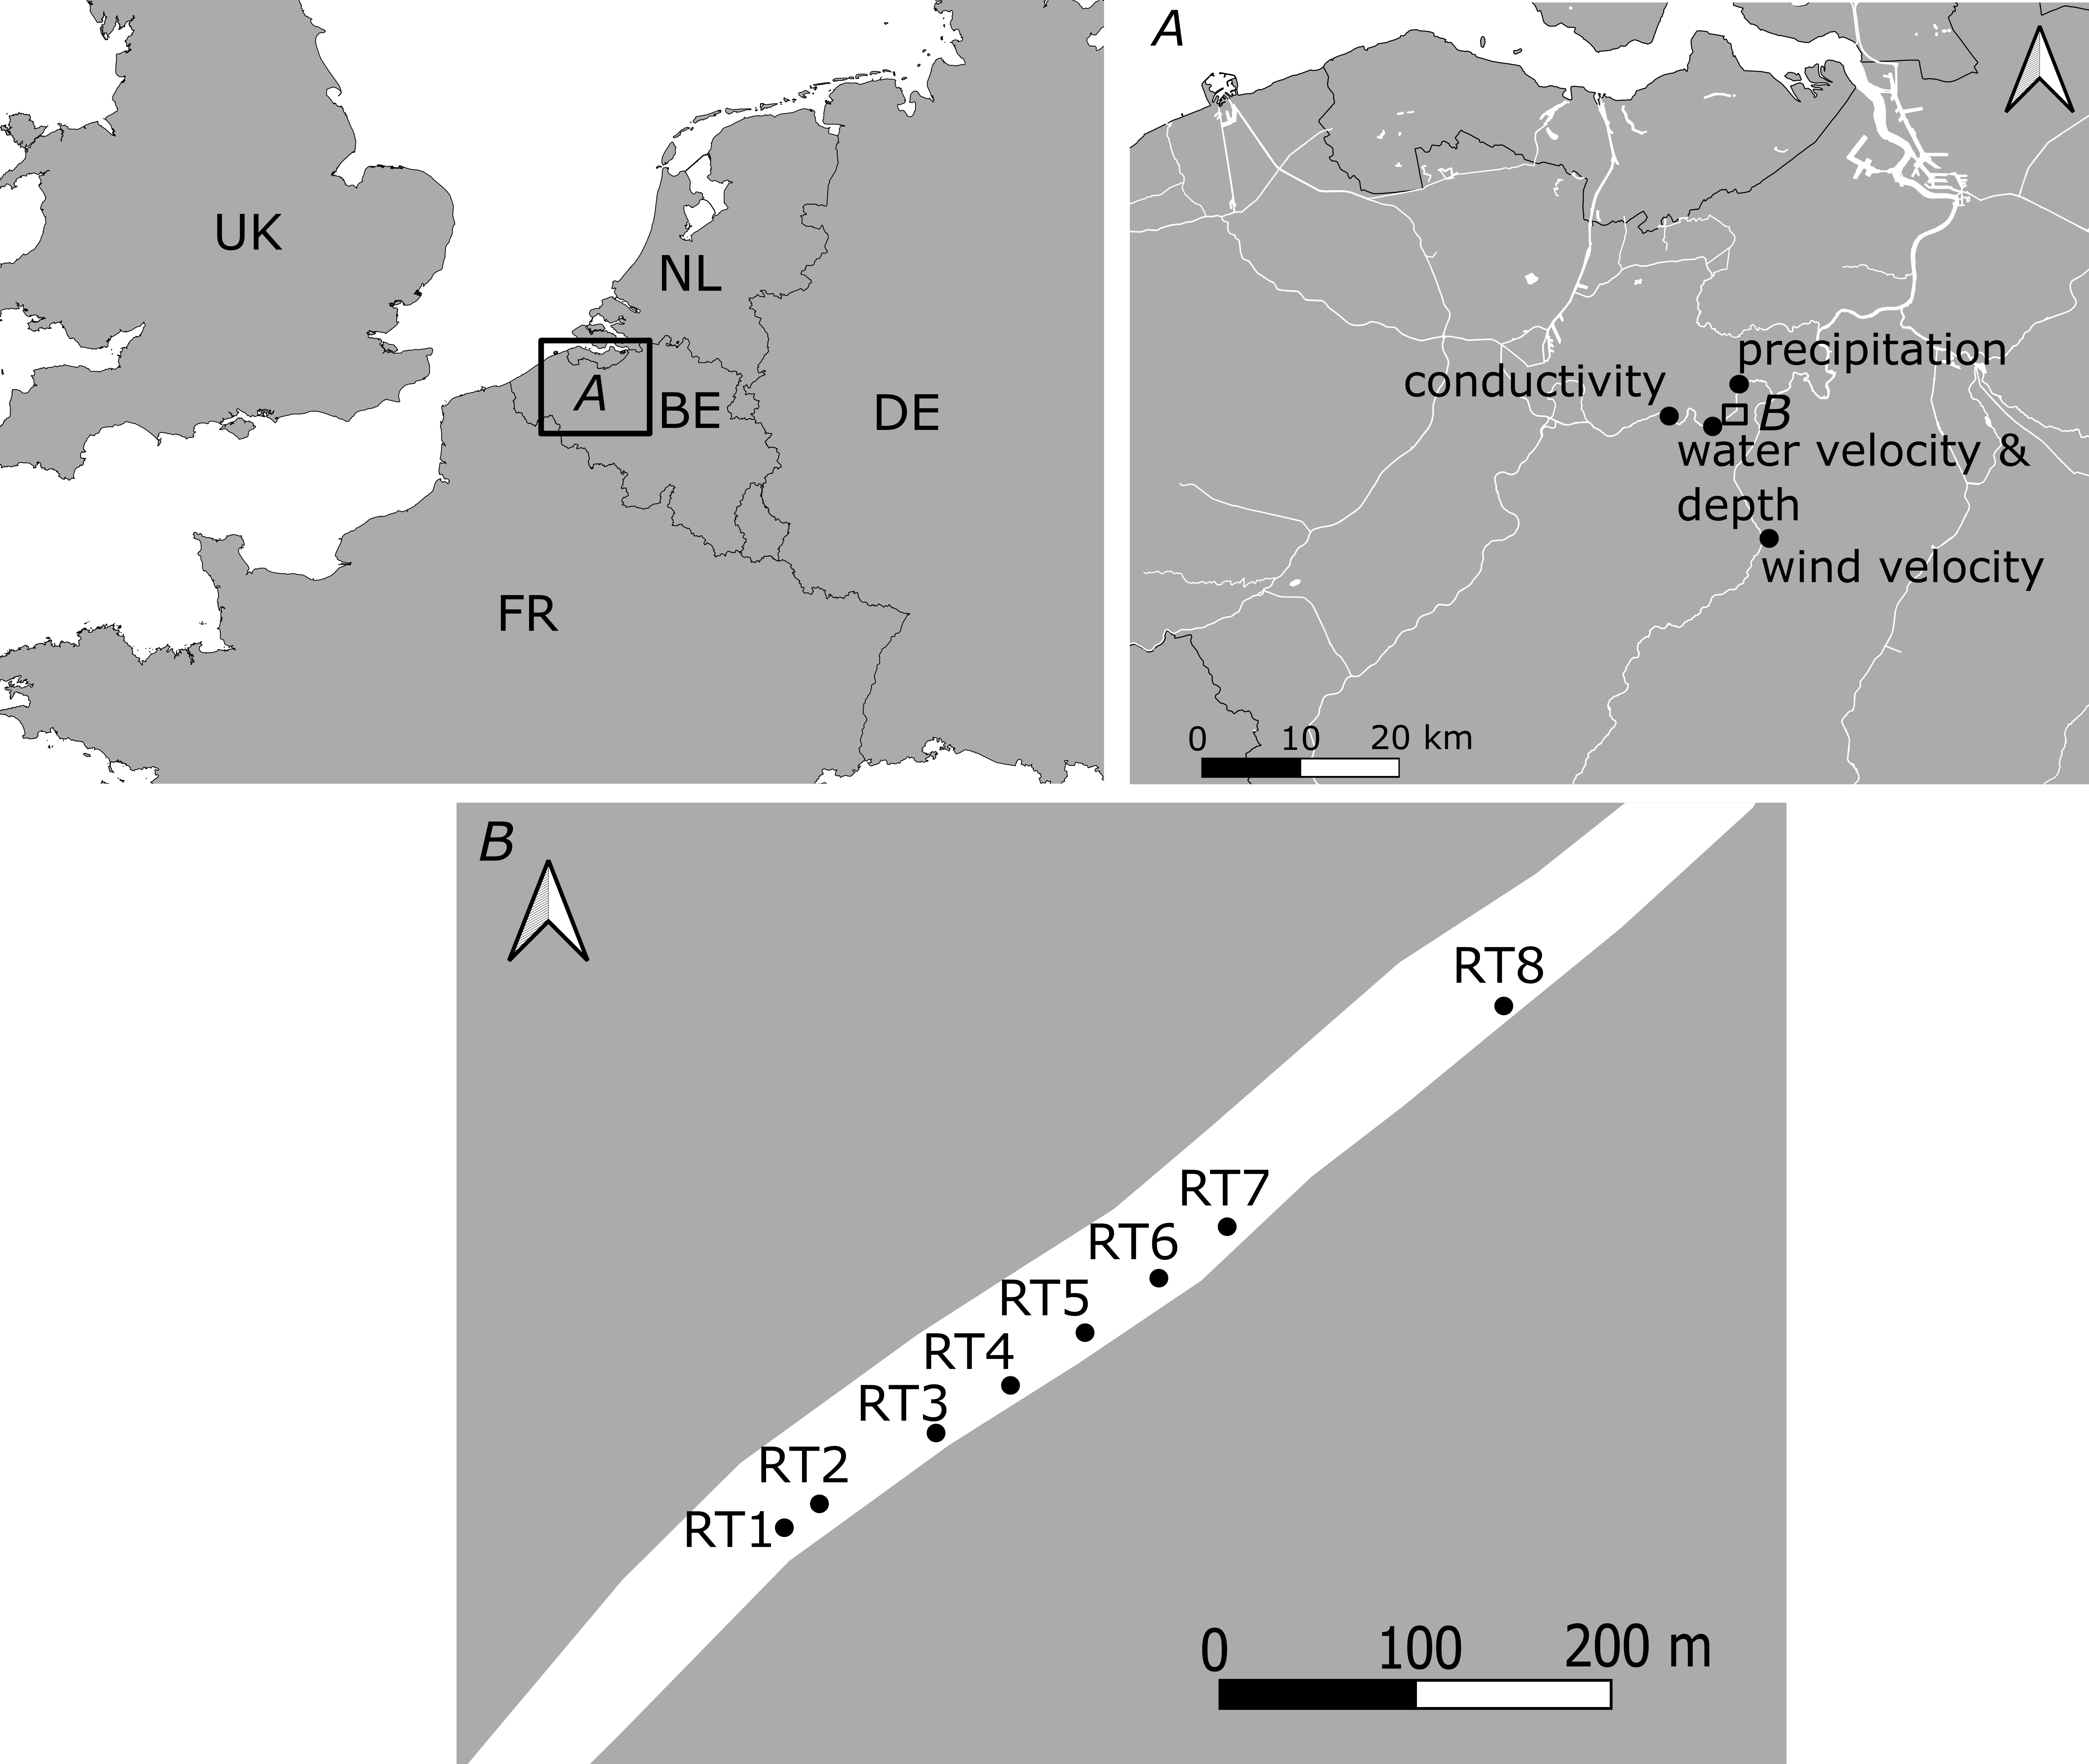
\includegraphics[width=0.85\textwidth]{study_area}
  \caption{\csentence{Depiction of the study area at different scales} In A, the site at which the receivers were placed (B) and the measurement locations for the electrical conductivity, precipitation, water velocity, water depth and wind velocity are depicted. In B, a more detailed depiction of the site with receivers is given, ranging from the first receiver, Rt1, to the last one, Rt8.}
  \label{fig:study_area}
\end{figure}

\begin{figure}[h!]
  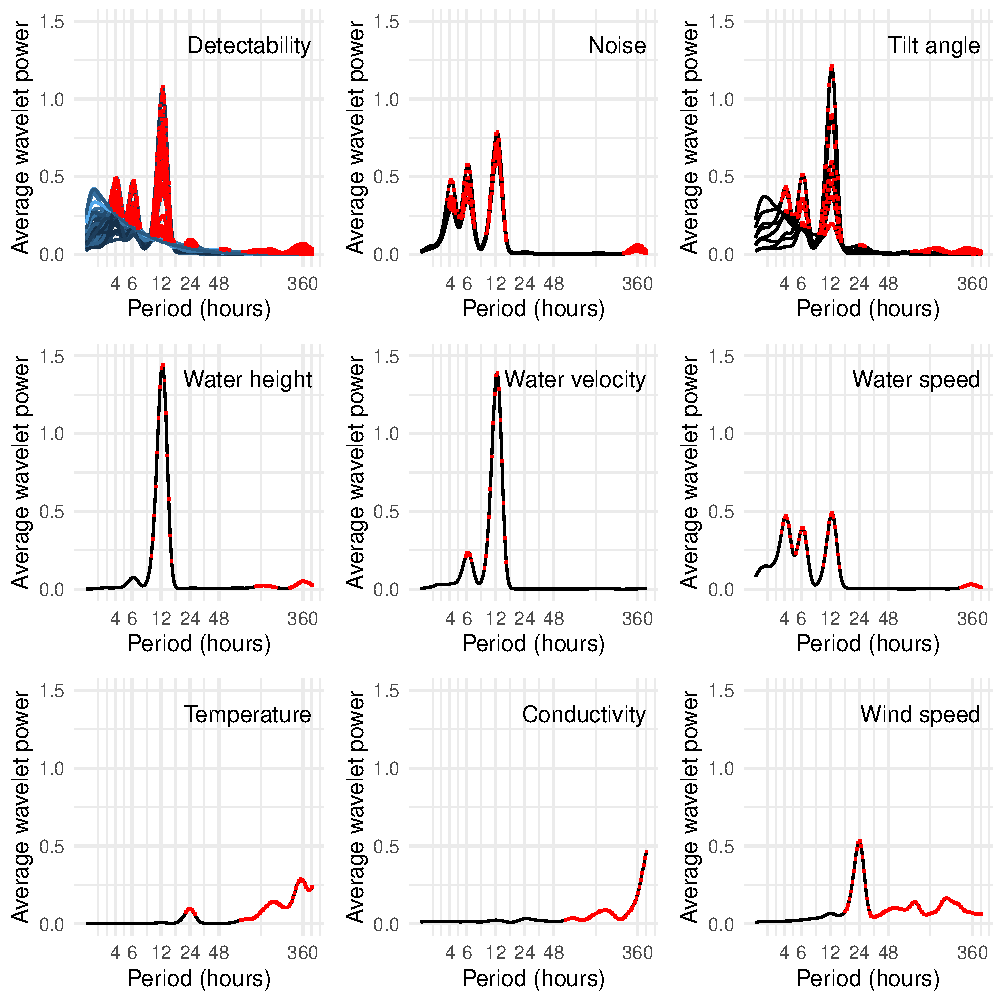
\includegraphics[width=0.85\textwidth]{singleWaveletAverageAll}
  \caption{\csentence{Average wavelet power in function of period (hours) for different variables.}
      For the performance all different distances between receivers are depicted. Darker blue colors represent smaller distances. For the tilt angle and ambient noise measurements, the different measuring receivers are depicted. Significant values (p$<$0.05) are depicted with red dots.}
  \label{fig:singleWaveletAverageAll}
\end{figure}

\begin{figure}[h!]
  \includegraphics[width=0.85\textwidth]{psem5}
  \caption{\csentence{pSEM model with depiction of the different sub-models (i.e. performance, noise and tilt angle).}
      The width of the arrows represents the standardized estimate of the relationship which is a measure of its relative importance.}
  \label{fig:psem5}
\end{figure}

\begin{figure}[h!]
  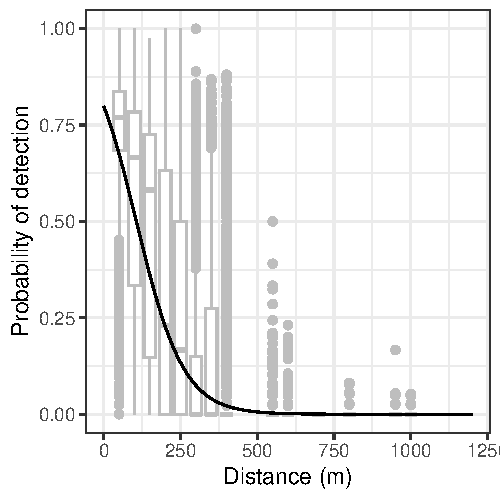
\includegraphics[width=0.42\textwidth]{logit_distance_plot.pdf}
  \caption{\csentence{Detection probability in function of the distance between receiver and transmitter.}
      Measurements (boxplots) and estimates (line) of detection probability in function of distance are depicted. The detection probability was estimated using the developed logistic submodel of the pSEM under average conditions of all other explanatory variables of the model.}
  \label{fig:logit_distance_plot}
\end{figure}

\begin{figure}[h!]
  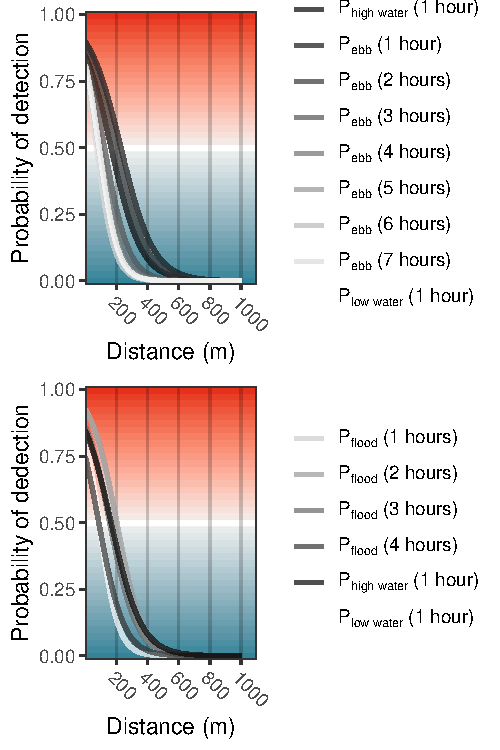
\includegraphics[width=0.42\textwidth]{DR_tide}
  \caption{\csentence{Detection probability in function of the distance between receiver and transmitter for different tidal phases.}
      The tidal cycle was subdivided in hourly tidal phases. Each curve represents the detection probability (P) for each subsequent hourly tidal phase. The top and bottom panel depict the detection probability during ebb and flood, respectively. No distinction was made between neap tide, spring tide or intermediate tide. The detection probability was estimated using the developed logistic submodel of the pSEM under median conditions of noise, water depth and tilt angle for all the considered tidal phases. R code to create this figure was adapted from \cite{Goossens2022TakingAssessments}. A larger version of this figure is provided in the Supplementary Information.}
  \label{fig:DR_tide}
\end{figure}

\begin{figure}[h!]
  \includegraphics[width=0.84\textwidth]{DR_tide_circ}
  \caption{Detection probability in function of the distance between receiver and transmitter for different hourly tidal phases. The tidal cycle was subdivided in hourly tidal phases. Each plot represents a subsequent hourly tidal phase. No distinction was made between neap tide, spring tide or intermediate tide. The detection probability was estimated using the developed logistic submodel of the pSEM under median conditions of noise, water depth and tilt angle for all the considered tidal phases. For each tidal phase the distance at which the detection probability was 50\% was given (D50). HW and LW stand for high water and low water respectively. R code to create this figure was adapted from \cite{Goossens2022TakingAssessments}.}
  \label{fig:DR_tide_circ}
\end{figure}

\begin{figure}[h!]
  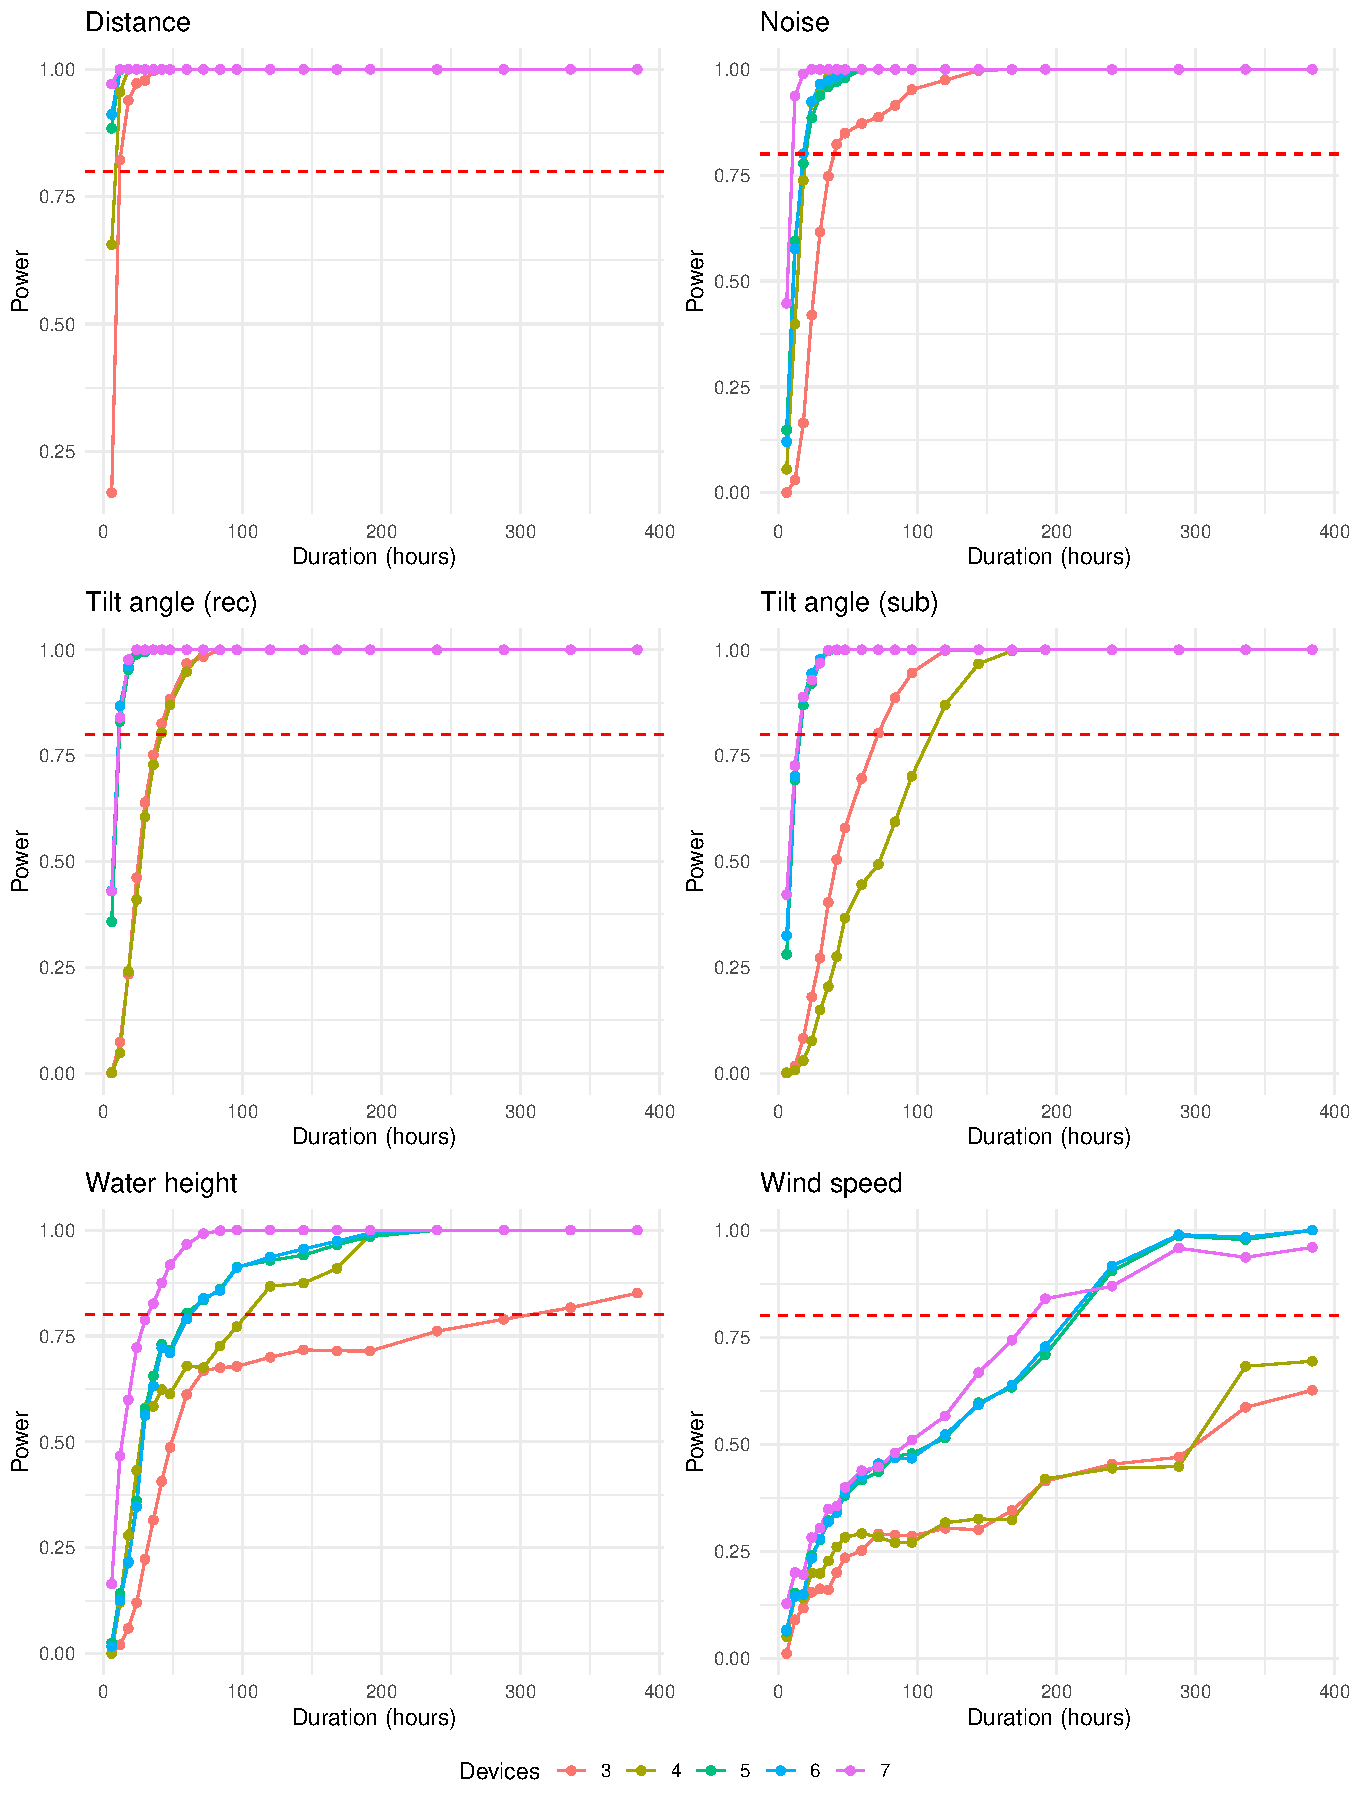
\includegraphics[scale=0.5]{Power_agg}
  \caption{\csentence{Statistical power analysis for the assessment of the drivers behind the performance based on the aggregated data without Rt6.}
      The statistical power is given in function of the duration of the experiment. The different colored lines represent scenarios with different numbers of receivers with built-in transmitters. The horizontal red dashed line represents the threshold of 0.8 at which the power is considered sufficient. }
  \label{fig:Power_agg}
\end{figure}



%%%%%%%%%%%%%%%%%%%%%%%%%%%%%%%%%%%
%%                               %%
%% Tables                        %%
%%                               %%
%%%%%%%%%%%%%%%%%%%%%%%%%%%%%%%%%%%

%% Use of \listoftables is discouraged.
%%
\section*{Tables}

\begin{table}[]
\centering
\caption{Technical details and placement details of the receivers (Rec) with built-in tags. The average (standard deviation) values of the hourly ambient noise (mV), tilt angle ($^\circ$) measurements and depth (m) are given. Dist.: distance (m). RBI: random burst interval (sec). Power output is expressed in dB. The VR2Tx combines a VR2W receiver with a built-in V16 transmitter. The VR2AR combines an acoustic release with a VR2Tx.}
\label{tab:tech}
\begin{tblr}{
  hline{1-2,10} = {-}{},
}
Rec & {Dist.\\(m)} & Code         & {Noise\\(mV)} & {Tilt angle\\($^\circ$)} & {RBI\\(sec)} & {Depth\\(m)} & {Power\\(dB)} \\
Rt1 & 0            & VR2Tx-480873 & 392 (149)     & 15 (15)          & 60-120       & 1.98 (1.13)  & 142 (L)          \\
Rt2 & 50           & VR2Tx-480874 & 376 (147)     & 21 (19)          & 60-120       & 1.83 (1.09)  & 142 (L)          \\
Rt3 & 200          & VR2Tx-480875 & 370 (136)     & 30 (4)           & 60-120       & 1.65 (1.02)  & 142 (L)          \\
Rt4 & 300          & VR2Tx-480876 & 357 (135)     & 20 (10)          & 540-660      & 2.20 (1.14)  & 142 (L)          \\
Rt5 & 400          & VR2Tx-480877 & 341 (127)     & 23 (6)           & 60-120       & 3.93 (1.14)  & 142 (L)          \\
Rt6 & 500          & VR2Tx-480878 & 316 (116)     & 18 (7)           & 60-120       & 3.89 (1.14)  & 142 (L)          \\
Rt7 & 600          & VR2AR-546043 & 344 (121)     & 51 (5)           & 540-660      & 1.71 (1.05)  & 142 (L)          \\
Rt8 & 1000         & VR2AR-546044 & 473 (166)     & 28 (12)          & 540-660      & 2.02 (1.13)  & 142 (L)          
\end{tblr}
\label{tab:tech}
\end{table}

\begin{table}[]
\centering
\caption{pSEM model output for aggregated data without Rt6. For the different sub-models (i.e. performance (Perf.), noise and tilt angle), for each variable, the coefficient estimates (Est), standard error (SE), critical value (Crit.Value), p-value and standardized estimates (Std.Est) are given.}
\begin{tabular}{llrrrrr}
\hline
Response                       & Predictor               & Est     & SE     & Crit.Value   & p-value      & Std.Est \\ \hline
\multirow{8}{*}{Perf.} & Distance                & -3.5378 & 0.0480 & -73.6953 & $<$0.0001            & -0.7479 \\
                               & Noise                   & -1.1846 & 0.0413 & -28.6946 & $<$0.0001            & -0.2504 \\
                               & Tilt angle (rec)        & -0.4859 & 0.0173 & -28.0736 & $<$0.0001            & -0.1027 \\
                               & Tilt angle (sub)        & -0.4361 & 0.0178 & -24.4391 & $<$0.0001            & -0.0922 \\
                               & Water depth (sub)      & 0.7096  & 0.0282 & 25.1729  & $<$0.0001            & 0.1500    \\
                               & Wind speed              & -0.1634 & 0.0149 & -10.9844 & $<$0.0001            & -0.0345 \\
                               & Distance * Water depth & 0.6283  & 0.0328 & 19.1276  & $<$0.0001            & 0.1228  \\
                               & Distance * Noise        & -0.4859 & 0.0437 & -11.1115 & $<$0.0001            & -0.1090  \\ \hline
\multirow{7}{*}{Noise}         & Water speed          & 0.7860  & 0.0.0025 & 313.4190 & $<$0.0001            & 0.7860  \\
                               & Water depth            & -0.3124 & 0.0030 & -104.6445 & $<$0.0001            & -0.3124 \\
                               & Precipitation           & 0.0920  & 0.0024 & 38.8070  & $<$0.0001            & 0.0920  \\
                               & Wind speed              & 0.0145  & 0.0024 & 6.0430   & $<$0.0001            & 0.0145  \\
                               & Tilt angle              & 0.0449 & 0.0041 & 10.9782  & $<$0.0001            & 0.0449\\
                               & Water depth * speed  & -0.1030  & 0.0023 & -44.4692   & $<$0.0001            & -0.1057  \\ \hline
\multirow{3}{*}{Tilt angle}    & Water speed          & 0.1637  & 0.0025 & 66.1016  & $<$0.0001            & 0.1637  \\
                               & Water depth            & -0.0721 & 0.0031 & -23.4724 & $<$0.0001            & -0.0721 \\
                               & Wind speed              & 0.0416  & 0.0025 & 16.8743  & $<$0.0001            & 0.0416  \\ \hline
\end{tabular}
\label{tab:pSEM}
\end{table}

\begin{table}[]
\centering
\caption{R$^{2}$ of the sub-models of the pSEM for data without Rt6. The marginal R$^{2}$ comprises the variance explained only by fixed effects while the conditional R$^{2}$ comprises the variance explained by the entire sub-model, i.e., both fixed and random effects. The R$^{2}$ of the performance was determined using the McFadden method.}
\begin{tabular}{lll}
\hline
Response      & Marginal R$^{2}$ & Conditional R$^{2}$ \\ \hline
Performance & 0.57        & /              \\ 
Noise         & 0.61        & 0.71           \\ 
Tilt angle    & 0.03        & 0.71           \\ \hline
\end{tabular}
\end{table}

\begin{table}[]
\centering
\caption{Model output of the most parsimonious logistic model for the non-aggregated-data without Rt6 with as response the Bernoulli performance. For each variable, the coefficient estimate (Est), standard error (SE), z-value, and p-value are given.}
\begin{tabular}{lrrrr}
\hline
Predictor                                        & Est    & SE    & z-value      & p-value \\ \hline
(Intercept)                                      & -3.251                  & 0.004                  & -762.476                    & $<$0.001 \\
Distance                                         & -3.496                  & 0.005                  & -659.352                    & $<$0.001 \\
Water speed                                      & -0.941                  & 0.003                  & -366.237                    & $<$0.001 \\
Tilt angle (sub)                                 & -0.384                  & 0.003                  & -147.082                    & $<$0.001 \\
Water depth (rec)                                & 0.448                   & 0.002                  & 189.136                     & $<$0.001 \\
Tilt angle (rec)                                 & -0.577                  & 0.003                  & -184.318                    & $<$0.001 \\
Water depth (sub)                                & 0.546                   & 0.003                  & 215.572                     & $<$0.001 \\
Wind speed                                       & -0.287                  & 0.003                  & -109.307                    & $<$0.001 \\
Precipitation                                    & -0.270                   & 0.004                  & -64.826                     & $<$0.001 \\
Temperature                                         & 0.066                   & 0.002                  & 26.488                      & $<$0.001 \\
Current signal angle (180°)                      & -0.058                  & 0.005                  & -11.155                     & $<$0.001 \\
Angle wind cosine                                & -0.005                  & 0.002                  & -1.919                      & 0.055    \\
Angle wind sine                                  & -0.004                  & 0.001                  & -3.365                      & 0.001    \\
Distance * Water depth (rec)                     & 0.275                   & 0.003                  & 78.950                       & $<$0.001 \\
Distance * Water depth (sub)                     & 0.508                   & 0.004                  & 136.725                     & $<$0.001 \\
Distance * Water speed                           & -0.271                  & 0.003                  & -93.773                     & $<$0.001 \\
Distance * Tilt angle (sub)                      & -0.185                  & 0.003                  & -56.887                     & $<$0.001 \\
Distance * Wind speed                            & -0.155                  & 0.003                  & -46.212                     & $<$0.001 \\
Distance * Precipitation                         & -0.203                  & 0.005                  & -42.722                     & $<$0.001 \\
Distance * Tilt angle (rec)                      & -0.133                  & 0.004                  & -35.126                     & $<$0.001 \\
Tilt angle (rec) * Current signal angle   (180°) & 0.224                   & 0.003                  & 71.309                      & $<$0.001 \\
Tilt angle (sub) * Current signal angle   (180°) & -0.156                  & 0.003                  & -60.121                     & $<$0.001 \\
Distance * Temperature                              & 0.088                   & 0.003                  & 27.072                      & $<$0.001 \\
Distance * Current signal angle (180°)           & -0.080                   & 0.007                  & -12.313                     & $<$0.001 \\
water speed * Current signal angle   (180°)      & 0.015                   & 0.003                  & 5.573                       & $<$0.001 \\
Wind speed * Angle wind sine                     & 0.007                   & 0.001                  & 5.344                       & $<$0.001 \\
Wind speed * Angle wind cosine                   & -0.007                  & 0.001                  & -4.796                      & $<$0.001 \\
Distance * Angle wind cosine                     & 0.012                   & 0.003                  & 3.967                       & $<$0.001 \\ \hline
\end{tabular}
\label{tab:GLM_bin}
\end{table}

\begin{table}[]
\centering
\caption{Per tidal phase the D50 (distance at which the detection probability was 50\%), median noise, median water depth, median tilt angle and median water speed are given. The tidal cycle was subdivided in hourly tidal phases. No distinction was made between neap tide, spring tide or intermediate tide. The detection probability was estimated using the developed logistic submodel of the pSEM under median conditions of noise, water depth and tilt angle for all the considered tidal phases. For each tidal phase the distance at which the detection probability was 50\% was given.}
\begin{tabular}{lrrrrrr}
\hline
\begin{tabular}[l]{@{}l@{}}Phase\\ (hours)\end{tabular} & \begin{tabular}[r]{@{}l@{}}D50\\ (m)\end{tabular} & \begin{tabular}[r]{@{}l@{}}Noise\\ (mV)\end{tabular} & \begin{tabular}[r]{@{}l@{}}Water\\ depth\\ (m)\end{tabular} & \begin{tabular}[r]{@{}l@{}}Tilt\\ angle\\ ($^\circ$)\end{tabular} & \begin{tabular}[r]{@{}l@{}}Water\\ velocity\\ (m/s)\end{tabular} \\
\hline
HW (1)                                                  & 171                                               & 326.80                                             & 3.60                                                        & 19.00                                                     & -0.65                                                            \\
Ebb (1)                                                 & 229                                               & 224.35                                             & 3.28                                                        & 18.00                                                     & 0.11                                                             \\
Ebb (2)                                                 & 200                                               & 223.40                                             & 2.72                                                        & 21.00                                                     & 0.62                                                             \\
Ebb (3)                                                 & 123                                               & 370.00                                             & 2.30                                                        & 23.00                                                     & 0.72                                                             \\
Ebb (4)                                                 & 100                                               & 443.20                                             & 1.81                                                        & 23.00                                                     & 0.72                                                             \\
Ebb (5)                                                 & 89                                                & 468.95                                             & 1.35                                                        & 24.00                                                     & 0.71                                                             \\
Ebb (6)                                                 & 83                                                & 482.25                                             & 0.92                                                        & 25.00                                                     & 0.70                                                             \\
Ebb (7)                                                 & 71                                                & 472.15                                             & 0.52                                                        & 29.00                                                     & 0.68                                                             \\
LW (1)                                                  & 88                                                & 418.40                                             & 0.46                                                        & 28.00                                                     & 0.64                                                             \\
Flood (1)                                               & 189                                               & 193.45                                             & 0.88                                                        & 21.25                                                     & 0.04                                                             \\
Flood (2)                                               & 203                                               & 192.90                                             & 1.51                                                        & 20.00                                                     & -0.38                                                            \\
Flood (3)                                               & 157                                               & 283.45                                             & 2.46                                                        & 23.00                                                     & -0.66                                                            \\
Flood (4)                                               & 88                                                & 474.00                                             & 3.32                                                        & 23.00                                                     & -0.88                                                            \\
HW (1)                                                  & 171                                               & 326.80                                             & 3.60                                                        & 19.00                                                     & -0.65                                                          \\ \hline
\end{tabular}
\label{tab:DR_tide}
\end{table}

\begin{table}[]
\centering
\caption{Required number of days to reach a statistical power of 80 \% for different variables and different numbers of receivers.}
\begin{tabular}{lrrrrr}
\hline
\multirow{2}{*}{Variables} & \multicolumn{5}{c}{Number of receivers} \\ 
                           & 3       & 4       & 5     & 6     & 7     \\ \hline
Noise                      & 1.75    & 0.75    & 0.75  & 0.75  & 0.50  \\
Distance                   & 0.50    & 0.25    & 0.25  & 0.25  & 0.25  \\
Tilt angle   (rec)         & 1.75    & 1.75    & 0.50  & 0.50  & 0.50  \\
Tilt angle   (sub)         & 3.00    & 5.00    & 0.75  & 0.75  & 0.50  \\
Water depth                & 12.00   & 4.00    & 2.50  & 2.50  & 1.25  \\
Wind speed                 & 16.00   & 16.00   & 8.00  & 8.00  & 8.00  \\ \hline
\end{tabular}
\label{tab:power}
\end{table}

%%%%%%%%%%%%%%%%%%%%%%%%%%%%%%%%%%%
%%                               %%
%% Additional Files              %%
%%                               %%
%%%%%%%%%%%%%%%%%%%%%%%%%%%%%%%%%%%

% \section*{Additional Files}
%   \subsection*{Additional file 1 --- Methodological aspects}
%   \label{ad:Methodological aspects}
%     % Additional file descriptions text (including details of how to
%     % view the file, if it is in a non-standard format or the file extension).  This might
%     % refer to a multi-page table or a figure.
    

%   \subsection*{Additional file 2 --- Sample additional file title}
%     Additional file descriptions text.


\end{backmatter}
\end{document}
